% -*- mode: noweb; noweb-default-code-mode: R-mode; -*-
\documentclass{article}
\usepackage{url}
\usepackage{amsfonts}

%\IfFileExists{url.sty}{\usepackage{url}}
 %                    {\newcommand{\url}{\text}}
                     
                     {\newcommand{\email}{\text}}

\usepackage{subfigure}
\usepackage[pdftex]{graphicx}
%\Keywords{Google map tiles, Google static maps, map coordinates}

%\Abstract{

%\usepackage{Sweave}
\begin{document}

%\VignetteIndexEntry{RgoogleMaps: An R Package for plotting on Google map tiles within R}
%\VignetteDepends{RgoogleMaps}
%\VignetteKeywords{Google Static Maps, coordinate transformation, map tiles, R, S}
%\VignettePackage{RgoogleMaps}

\title{Plotting on Google Static Maps in R}
\author{Markus Loecher\\  Sense Networks \\  \it{markus@sensenetworks.com}}

\maketitle
\noindent
The Google Static Maps API (\url{http://code.google.com/apis/maps/documentation/staticmaps/}) lets you embed a Google Maps image on your webpage without requiring JavaScript or any dynamic page loading. The Google Static Map service creates your map based on URL parameters sent through a standard HTTP request and returns the map as an image you can display on your web page.

\noindent Note: The Google Static Maps API does NOT require a Maps API key any longer. 
%If you haven't already done so, sign up for a free API key at \url{http://code.google.com/apis/maps/signup.html}.

\noindent This package serves two purposes:
\begin{itemize}
\item  Provide a comfortable R interface to query the Google server for static maps 
\item Use the map as a background image to overlay plots within R. This requires proper coordinate scaling.
\end{itemize}
\begin{figure}[ht]
\subfigure{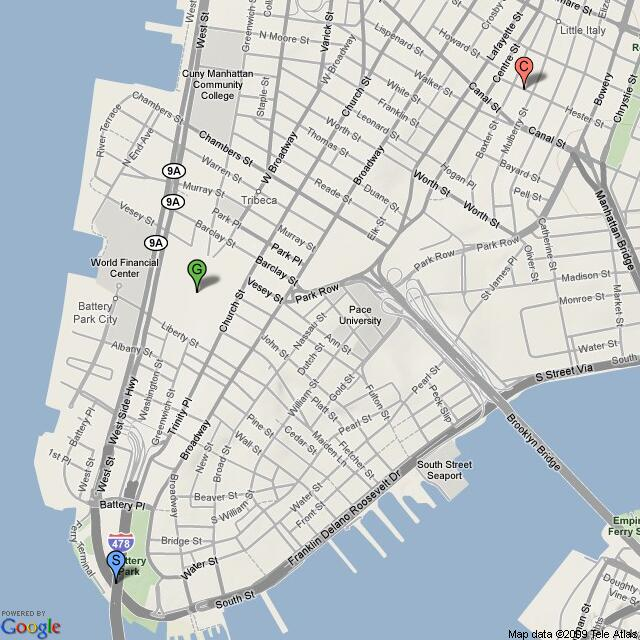
\includegraphics[width=.5 \textwidth]{MyTile1.jpg}}
\subfigure{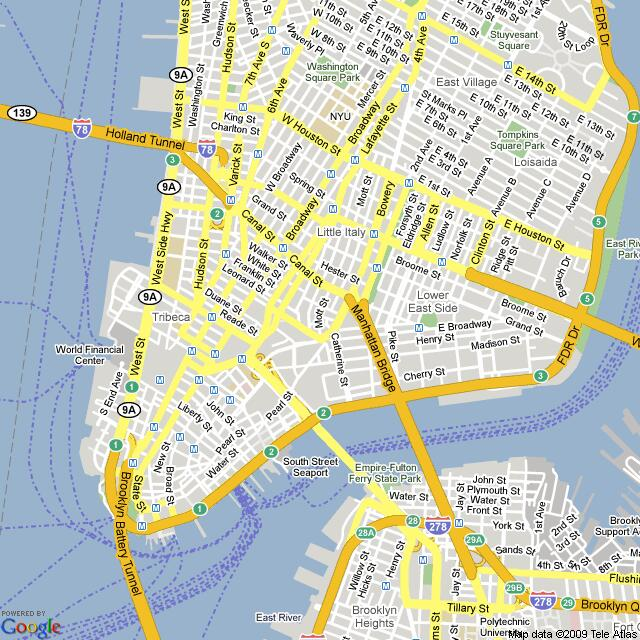
\includegraphics[width=.5 \textwidth]{MyTile2.jpg}}
    \caption{(a) Static map with markers, (b) Static (mobile) map}
\end{figure}

\noindent The first step naturally will be to download a static map from the Google server. A simple example (Fig 1a):
\begin{verbatim}
  MyMap <- GetMap(markers = 'color:blue|label:S|40.702147,-74.015794&markers=color:green|
           label:G|40.711614,-74.012318&markers=color:red|color:red|label:C|
           40.718217,-73.998284', destfile = "MyTile1.png")

\end{verbatim}
Of course, one can do without the markers and/or just pass a bounding box (Figs 1b and 2a):
\begin{verbatim}
  GetMap(center=c(40.714728,-73.99867), zoom =14, destfile = "MyTile2.png",
               maptype = "mobile");
  
  bb <- qbbox(c(40.702147,40.711614,40.718217),c(-74.015794,-74.012318,-73.998284), 
            TYPE = "all", margin = list(m=rep(5,4), TYPE = c("perc", "abs")[1]));
  MyMap <- GetMap.bbox(bb$lonR, bb$latR,destfile = "MyTile3.png", maptype = "satellite")
\end{verbatim}
\begin{figure}[ht]
\subfigure{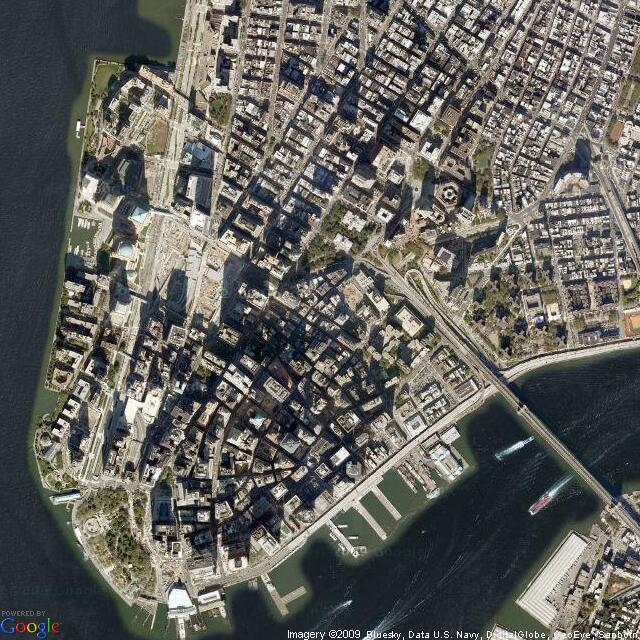
\includegraphics[width=.5 \textwidth]{MyTile3.jpg}}
\subfigure{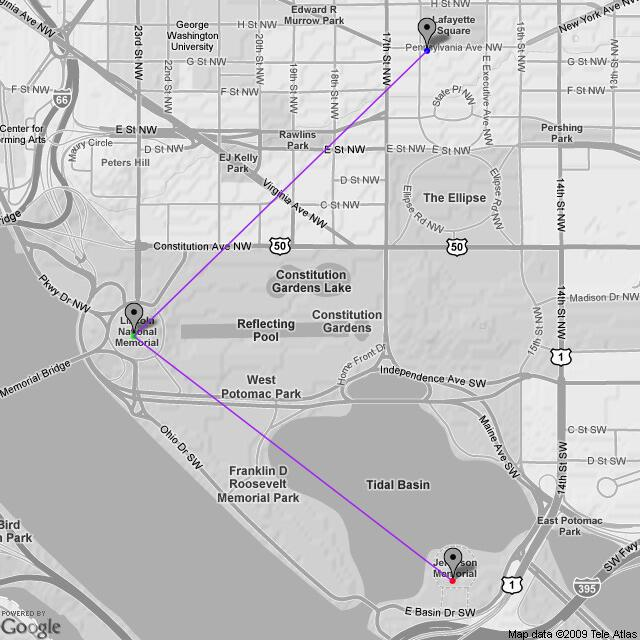
\includegraphics[width=.5 \textwidth]{OverlayTest.jpg}}
    \caption{(a) Static (satellite) map, (b)Testing point overlay}
\end{figure}

\noindent The function qbbox() basically computes a bounding box for the given lat,lon points with a few additional options such as quantile boxes, additional buffers, etc.
In order to plot the map we need the package $rgdal$.
We further need a way to change the current user coordinates, as set by par('usr') to our liking. The library $TeachingDemos$ contains a function $updateusr()$ that does exactly that. We took the liberty of including it in our package.

\noindent The function LatLon2XY(lat,lon,zoom) computes the coordinate transformation from lat/lon to map tile coordinates. 
It returns the tile coordinates as well as the pixel coordinates within the Tile itself.
Thanks to Neil Young (see \url{http://groups.google.com/group/Google-Maps-API/browse_thread/thread/d2103ac29e95696f?hl=en}) for providing the formulae used in that function

\noindent The choice of a proper zoom value is made easy via the function $MaxZoom()$ which finds the maximum zoom level that fits the provided lat/lon ranges obeying the max size limitation of $640 \times 640$ pixels.

\noindent The main function that overlays points (can easily be extended to lines or any other object) is $PlotOnStaticMap()$.
The following simple sequence of calls serves to test the coincidence of the markers placed by Google and the corresponding points overlaid by $PlotOnStaticMap()$, see Fig. 2b. Note that we convert the map to grayscale first to make the colored points more discernible.
\begin{verbatim}
#Define the markers:
  mymarkers <- cbind.data.frame(lat = c(38.898648,38.889112, 38.880940), 
      lon = c(-77.037692, -77.050273, -77.03660), size =  c('tiny','tiny','tiny'), 
      col = c('blue', 'green', 'red'), char = c('','',''));

#get the bounding box:
  bb <- qbbox(lat = mymarkers[,"lat"], lon = mymarkers[,"lon"])
#download the map:
  MyMap <- GetMap.bbox(bb$lonR, bb$latR, destfile = "DC.png", GRAYSCALE =T,
                markers = mymarkers);
#determine the max zoom, so that all points fit on the plot
# (not necessary in this case):  
   zoom <- min(MaxZoom(latrange=bb$latR,lonrange=bb$lonR));
 #plot:
 png("OverlayTest.png",640,640);
  tmp <- PlotOnStaticMap(MyMap,lat = mymarkers[,"lat"], lon = mymarkers[,"lon"], 
         cex=1.5,pch=20,col=c('blue', 'green', 'red'), add=F);
  tmp <- PlotOnStaticMap(MyMap,lat = mymarkers[,"lat"], lon = mymarkers[,"lon"], 
       col=c('purple'), add=T, FUN = lines, lwd = 2)
  dev.off()
\end{verbatim}

\noindent We have recently added the ability to (i) query the OpenStreetMap \begin{verbatim} (http://www.openstreetmap.org/) \end{verbatim} server for map tiles and (ii) to display axis on the image plot. In both cases, we felt that it was sensible to not transform the coordinates to Google's XY format but to instead leave the lat/lon coords as is. The advantage is that no coordinate transformation is needed to overlay points and lines on the map, so the plain R points() and lines() functions will work just fine. This convenience comes at the cost of the obvious misalignment due to lat/lon distortion which maybe slight or substantial, depending on the scale, so we provide a toggle to turn this on or off.
For OSM-type maps, the argument {\it TrueProj} is set to FALSE automatically.  
The following simple example is shown in Figure 3.

\begin{verbatim}
PrincetonMap <- GetMap.OSM(lonR= c(-74.67102, -74.63943), 
latR = c(40.33804,40.3556), scale = 7500, destfile = "Princeton.png");
PlotOnStaticMap(PrincetonMap, axes = TRUE, mar = rep(4,4));
\end{verbatim}
\begin{figure}[thb]
\centering
   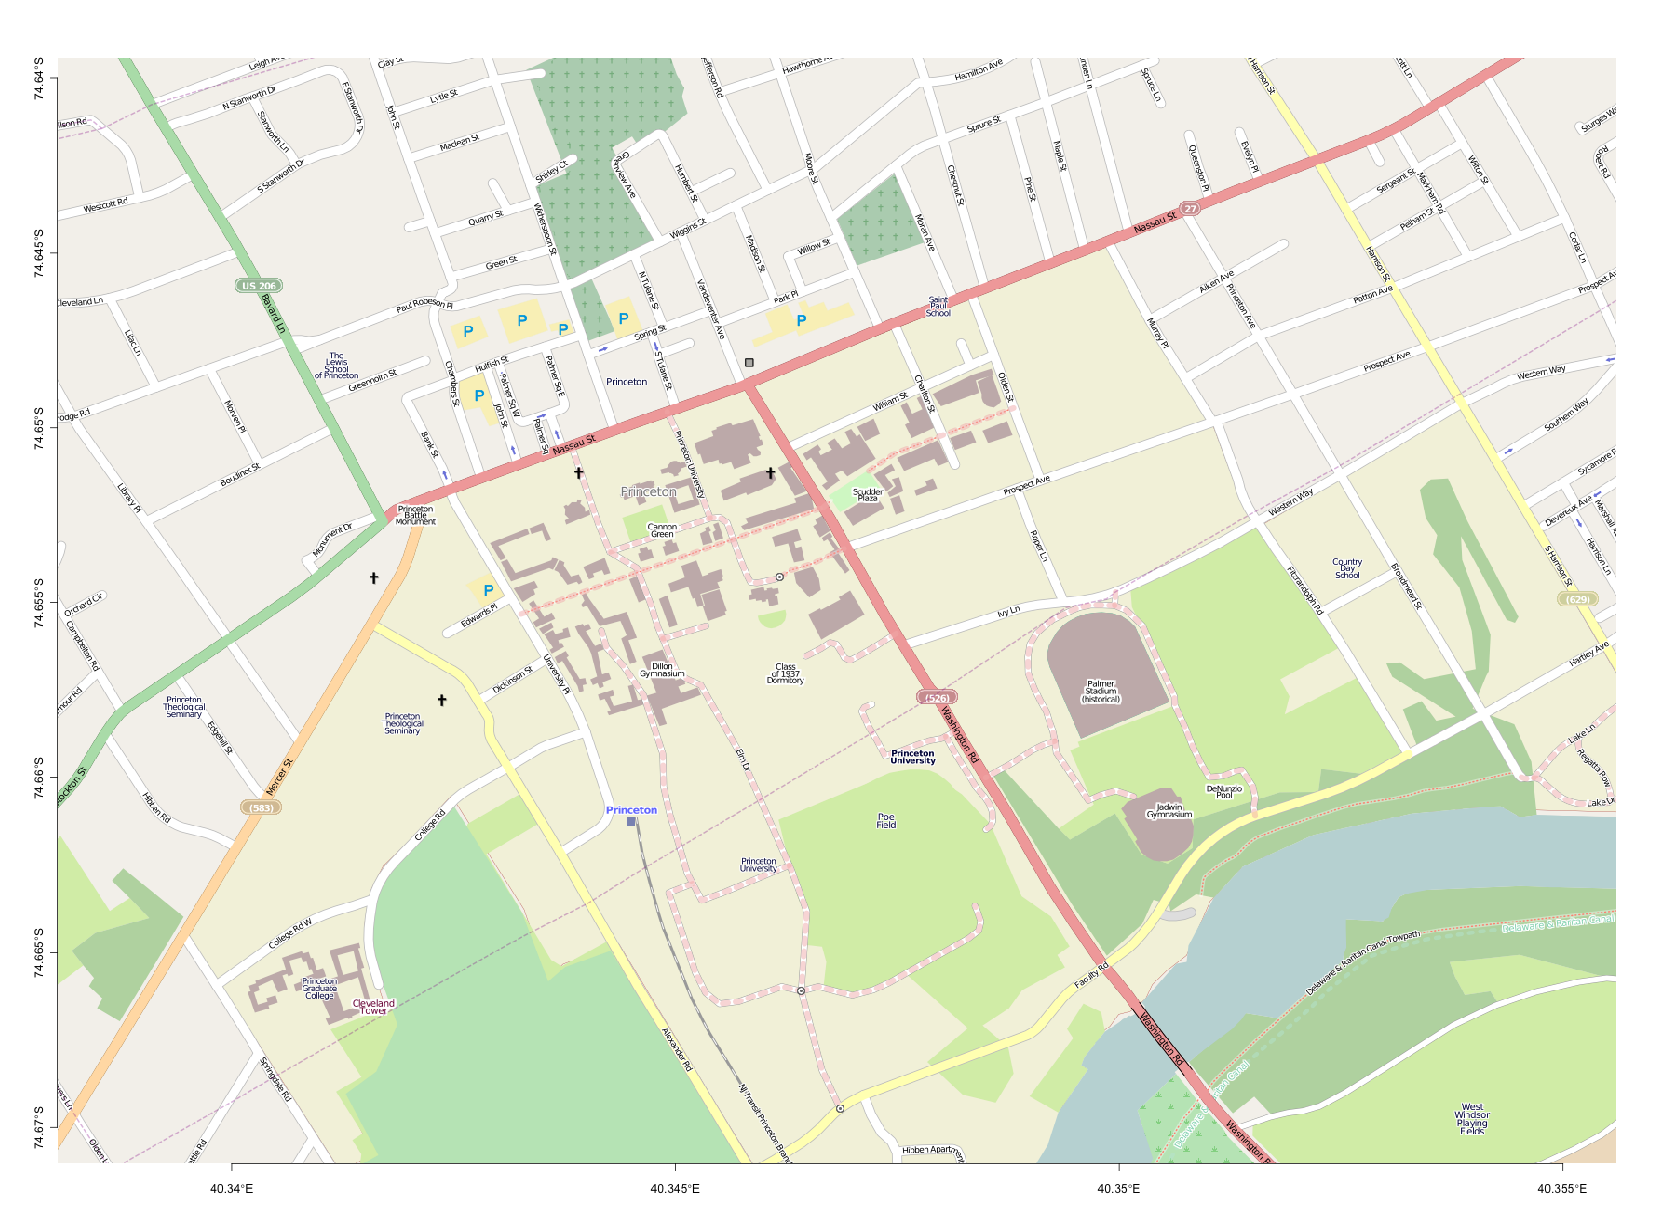
\includegraphics[width = .975 \textwidth]{Princeton.png}
    \caption{Princeton, NJ as displayed in OpenStreetMap}
\end{figure}

\noindent And lastly, one more fun example. The Coso geothermal field (e.g. \url{http://geology.about.com/od/mineral_resources/ig/cosogeotherm/}) is America's second-largest producer of geothermal electricity, with a continuous output of 270 megawatts. It relies on superheated groundwater that boils into steam at less than 2 kilometers depth, thus it is classified as a hot-water field. (The Geysers, world's largest geopower site in northern California, produces pure steam.)

\noindent Geothermal power has been produced at Coso since 1987 by a private contractor for the U.S. Navy, which acquired the land in 1943 as part of the China Lake Naval Air Weapons Station. The power is sold into the local utility grid.

\noindent The package $geomapdata$ contains a dataframe $cosomap$ which contains location information on the "Coso Geothermal Region Faults and Geology".
The following commands plot the fault lines on a Google map tile (Fig. 4):
\begin{verbatim}
 library(geomapdata);
 bb <- qbbox(lon=cosomap$POINTS$lon-360,lat=cosomap$POINTS$lat)
 MyMap <- GetMap.bbox(bb$lonR, bb$latR,destfile = "Coso.png", 
                     maptype="satellite",zoom=11)
 tmp <- PlotOnStaticMap(MyMap,lon=cosomap$POINTS$lon-360,
             lat=cosomap$POINTS$lat, pch=20,cex = .5,col='red',verbose=0);
\end{verbatim}

\begin{figure}[thb]
\centering
   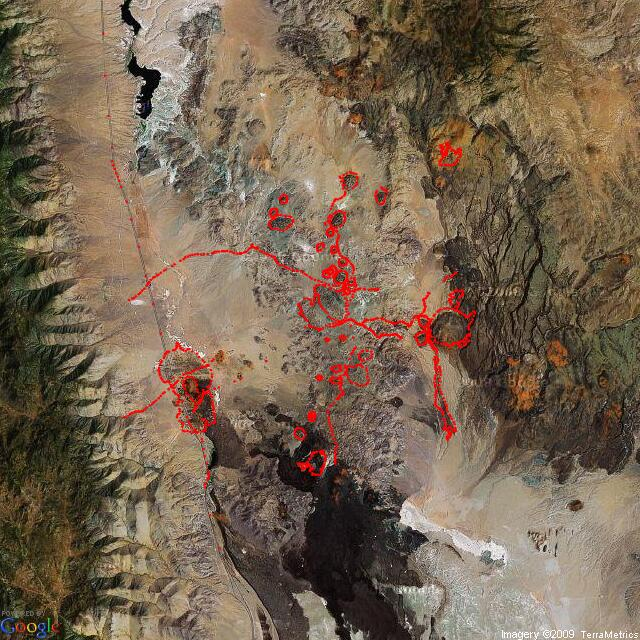
\includegraphics[width = .975 \textwidth]{Coso.jpg}
    \caption{Coso Geothermal Region Faults}
\end{figure}


\noindent The bulk of the remaining code deals mainly with efficiency as well as exploiting the many features offered by the Google Maps API.
For repeated plotting on the same static map, the user most likely does not want to request the same map over and over again. 
By setting $NEWMAP = F$ in $GetMap.bbox()$ the function itself reads the map straight from the file specified by $destfile$.
Furthermore, in order to not repeatedly read the map from a file, it can be stored and passed to most functions in the list $MyMap$ that additionally contains information on the zoom level and the center.

Future versions will include the ability to handle png files in addition to jpg.

\noindent In terms of features, the Static Maps API defines map images using the following URL parameters:
\begin{itemize}
    \item center (required if markers not present) defines the center of the map, equidistant from all edges of the map. This parameter takes a comma-separated {latitude,longitude} pair (e.g. "40.714728,-73.998672") identifying a unique location on the face of the earth. For more information, see latitudes and longitudes below.
    \item zoom (required if markers not present) defines the zoom level of the map, which determines the magnification level of the map. This parameter takes a numerical value corresponding to the zoom level of the region desired. For more information, see zoom levels below.
    \item size (required) defines the rectangular dimensions of the map image. This parameter takes a string of the form valuexvalue where horizontal pixels are denoted first while vertical pixels are denoted second. For example, 500x400 defines a map 500 pixels wide by 400 pixels high. If you create a static map that is 100 pixels wide or smaller, the "Powered by Google" logo is automatically reduced in size.
    \item format (optional) defines the format of the resulting image. By default, the Static Maps API creates GIF images. There are several possible formats including GIF, JPEG and PNG types. Which format you use depends on how you intend to present the image. JPEG typically provides greater compression, while GIF and PNG provide greater detail. For more information, see Image Formats.
    \item maptype (optional) defines the type of map to construct. There are several possible maptype values, including satellite, terrain, hybrid, and mobile. For more information, see Static Maps API Maptypes below.
    \item markers (optional) define one or more markers to attach to the image at specified locations. This parameter takes a string of marker definitions separated by the pipe character (|). Note that if you supply markers for a map, you do not need to specify the (normally required) center and zoom parameters. For more information, see Static Map Markers below.
    \item path (optional) defines a single path of two or more connected points to overlay on the image at specified locations. This parameter takes a string of point definitions separated by the pipe character (|). Note that if you supply a path for a map, you do not need to specify the (normally required) center and zoom parameters. For more information, see Static Map Paths below.
    \item span (optional) defines a minimum viewport for the map image expressed as a latitude and longitude pair. The static map service takes this value and produces a map of the proper zoom level to include the entire provided span value from the map's center point. Note that the resulting map may include larger bounds for either latitude or longitude depending on the rectangular dimensions of the map. If zoom is specified, span is ignored.
    \item frame (optional) specifies that the resulting image should be framed with a colored blue border. The frame consists of a 5 pixel, 55\% opacity blue border.
    \item hl (optional) defines the language to use for display of labels on map tiles. Note that this paramater is only supported for some country tiles; if the specific language requested is not supported for the tile set, then the default language for that tile set will be used.
    \item key (required) identifies the Maps API key for the domain on which this URL request takes place. If you don't have a Maps API key, you can sign up for one free.
    \item sensor (required) specifies whether the application requesting the static map is using a sensor to determine the user's location. This parameter is now required for all static map requests. For more information, see Specifying Locations below.
\end{itemize}

\section{Appendix: MapMath Details}

\noindent
We measure latitude and longitude in degrees but assume that the trigonometric functions used below expect units to be in radians.

\noindent
With   $\tilde{lat} = \pi \cdot lat /180$, the transformation from lat/lon to pixels is given by:
\begin{equation}   
\label{Eq1}
  \tilde{Y} = \frac{1}{2 \pi}  \log{\left( \frac{1 + \sin{(\tilde{lat})}}{1 -\sin{(\tilde{lat})} } \right)}
\end{equation} 
\begin{equation} 
\label{Eq2}  
  Y = 2^{zoom-1} * (1 - \tilde{Y}) ,  X = 2^{zoom-1} * (\tilde{X} + 1) 
\end{equation} 
The integer part of $X, Y$ specifies the tile, whereas the fractional part times $256$ is the pixel coordinate within the Tile itself:
\[
 x = 256 *(X- \lfloor{X}), y = 256 *(Y- \lfloor{Y})
\]
Inverting these relationships is rather straightforward.
Eq. (\ref{Eq1}) leads to 
\begin{equation}
  \tilde{lat} = 2 \pi n \pm  \sin^{-1}{\left( \frac{\exp{ 2 \pi \tilde{Y}} - 1}{\exp{ 2 \pi \tilde{Y}} + 1} \right)} + \pi  , n \in \mathbb{Z}
\end{equation}
whereas inverting Eqs. (\ref{Eq2})  gives
\[
\tilde{Y} = 1 - Y/2^{zoom-1} , \tilde{X} =  X/2^{zoom-1} - 1
\]
For longitude, the inverse mapping is much simpler:
Since $\tilde{X} = lon / 180 $, we get
 \[ 
lon =  180 \cdot \left( X/2^{zoom-1} - 1 \right).
\]
As a final remark, note that while latitude increases heading north, Google maps $Y$ coordinates move opposite, i.e. increase southward.



\end{document}


